\documentclass[8pt,a4paper]{article}
\usepackage[utf8]{inputenc}
\usepackage[spanish]{babel}
\usepackage{url}
\usepackage[hidelinks]{hyperref}
\usepackage{amsmath}
\usepackage{amsfonts}
\usepackage{amssymb}
\usepackage{amsthm}
\usepackage{siunitx}
\usepackage{mathtools}
\usepackage{graphicx}
\usepackage{subcaption}
\usepackage{float}
\usepackage{lipsum}
\usepackage{enumitem}
\usepackage{multicol}
\usepackage{caption}
\usepackage{balance}
\DeclareMathOperator{\expec}{E}
\DeclareMathOperator{\var}{Var}
\DeclareMathOperator{\cov}{Cov}
\newcommand{\Qf}{Q_{\text{final}}}
\newcommand{\defequal}{\vcentcolon =}

\newtheorem{thm}{Teorema}
\theoremstyle{definition}
\newtheorem{definition}{Definición}
\theoremstyle{remark}
\newtheorem{remark}{Observación}
\newtheorem*{remark*}{Observación}

% ====================================================================
% ======   Parámetros de configuración para mostrar código   =========
% ====================================================================
\usepackage{listings}
\usepackage{xcolor}

\definecolor{codegreen}{rgb} {0,0.6,0}
\definecolor{codegray}{rgb}  {0.5,0.5,0.5}
\definecolor{codepurple}{rgb}{0.58,0,0.82}
\definecolor{backcolour}{rgb}{0.95,0.95,0.92}

\lstdefinestyle{mystyle}{
    backgroundcolor=\color{backcolour},     % Indica el color de fondo; necesita que se añada \usepackage{color} o \usepackage{xcolor}
    commentstyle=\color{codegreen},         % Estilo de los comentarios
    keywordstyle=\color{magenta},           % Estilo de las palabras clave
    numberstyle=\tiny\color{codegray},      % Estilo para los números de línea
    stringstyle=\color{codepurple},         % Estilo de las cadenas de texto
    basicstyle=\ttfamily\footnotesize,      % Fija el tamaño del tipo de letra utilizado para el código
    %breakatwhitespace=false,                % Activarlo para que los saltos automáticos solo se apliquen en los espacios en blanco
    %breaklines=true,                        % Activa el salto de línea automático
    captionpos=b,                           % Establece la posición de la leyenda del cuadro de código
    keepspaces=true,                        % Mantiene los espacios en el texto. Es útil para mantener la indentación del código(puede necesitar columns=flexible).
    numbers=left,                           % Posición de los números de línea (none, left, right).
    numbersep=2pt,                          % Distancia de los números de línea al código
    showspaces=false,                       % Si se activa, muestra los espacios con guiones bajos; sustituye a 'showstringspaces'
    showstringspaces=false,                 % subraya solamente los espacios que estén en una cadena de esto
    showtabs=false,                         % si se activa muestra las tabulaciones que existan en cadenas de texto con guión bajo
    tabsize=2                               % Establece el salto de las tabulaciones a 2 espacios
}


% ====================================================================
% ======================    Parametros    ============================
% ====================================================================
\lstset{style=mystyle}

\newcommand{\celda}[1]{
	\begin{minipage}{2.5cm}
		\vspace{5mm}
		#1
		\vspace{5mm}
	\end{minipage}
}


\definecolor{azul}{rgb}{0.0, 0.53, 0.74}
\usepackage[left=2.00cm, right=2.00cm, top=2.00cm, bottom=2.00cm]{geometry}
\author{ABET23}
\title{Proyecto ABET}


\begin{document}
% ====================================================================
% ======================    ENCABEZADO    ============================
% ====================================================================
	\begin{figure}[H]
		\raggedright
		\hfill 
\includegraphics[scale=0.20]{escudouni.png}
	\end{figure}

	\vspace{7.5mm}
	
	\begin{center}
		{\Large \textbf{Compresión de imágenes: Una visión matemática y aplicada}}\\
		\vspace{2mm}
		{\large Alvaro P. Alvarado Lara (100\%)$^{1}$, Henry C. Ferreyra Cordero (100\%)$^{2}$, Yamil D. Aucca Quispe (100\%)$^{3}$, Julio A. Chumbimuni Ricci (100\%)$^{4}$ }\\
		\vspace{7.5mm}
		
		$^1$\textit{Facultad de ciencias, Universidad Nacional de Ingenier\'ia, e-mail: alvaro.alvarado.l@uni.pe} \\
		$^2$\textit{Facultad de ciencias, Universidad Nacional de Ingenier\'ia, e-mail: henry.ferreyra.c@uni.pe} \\
		$^3$\textit{Facultad de ciencias, Universidad Nacional de Ingenier\'ia, e-mail: yamil.aucca.q@uni.pe} \\
		$^4$\textit{Facultad de ciencias, Universidad Nacional de Ingenier\'ia, e-mail: julio.chumbimuni.r@uni.pe} \\
	\end{center}


% ====================================================================
% ======================      Abstract     ============================
% ====================================================================
	\begin{center}
		\textcolor{azul}{\rule{150mm}{0.5mm}}
	\end{center}		

	\begin{quotation}
    {\small
        %\begin{abstract}
        \begin{center}
            Resumen	
        \end{center}
        \vspace{0.3cm}
            La compresión de imágenes es una técnica fundamental en el procesamiento y almacenamiento de datos visuales. Este trabajo explora los fundamentos matemáticos de la compresión JPEG, centrándose en la Transformada Discreta del Coseno (DCT) como transformación lineal en espacios vectoriales. Se demuestra cómo bloques de imagen pueden modelarse como vectores en $\mathbb{R}^{64}$ y cómo la DCT actúa como isomorfismo lineal preservando la energía de la imagen. El análisis incluye verificaciones de axiomas de espacios vectoriales, propiedades de ortogonalidad y aplicaciones prácticas en compresión con pérdida.
        %\end{abstract}

        \vspace{2mm}

        \underline{\textbf{Palabras Claves:}}  \hspace{1mm} \textit{Compresión de imágenes, DCT, Álgebra Lineal, JPEG, espacios vectoriales.}
    }\\
    {\small
        \hspace*{0.5cm}
        \begin{center}
            Abstract
        \end{center}

            Image compression is a fundamental technique in visual data processing and storage. This work explores the mathematical foundations of JPEG compression, focusing on the Discrete Cosine Transform (DCT) as a linear transformation in vector spaces. We demonstrate how image blocks can be modeled as vectors in $\mathbb{R}^{64}$ and how the DCT acts as a linear isomorphism preserving image energy. The analysis includes verification of vector space axioms, orthogonality properties, and practical applications in lossy compression.

        \vspace{2mm}

        \underline{\textbf{Keywords:}}  \hspace{1mm} \textit{Image compression, DCT, Linear Algebra, JPEG, vector spaces.}
    }
    \end{quotation}

	\begin{center}
		\textcolor{azul}{\rule{150mm}{0.5mm}}
	\end{center}		

	\vspace{5mm}


% ====================================================================
% ======================     Contenido     ===========================
% ====================================================================
	\begin{multicols}{2}
	\begin{center}
    \section{Introducción}
    \end{center}

        \subsection{Breve historia y aplicaciones de la compresión de imágenes}
        
            La compresión de imágenes es una técnica fundamental en el procesamiento y almacenamiento de datos visuales. Su desarrollo se remonta a los años 1960, con los primeros algoritmos diseñados para transmitir imágenes vía satélite. Posteriormente, con la expansión de la computación personal y la digitalización de medios, surgió la necesidad de reducir el tamaño de los archivos sin comprometer su calidad perceptual.
            
            Durante los años 1980 y 1990, se formalizaron los primeros estándares de compresión con pérdida, entre los que destaca el formato JPEG (Joint Photographic Experts Group), basado en la Transformada Discreta del Coseno (DCT). Este formato se convirtió rápidamente en el estándar predominante para la compresión de imágenes fotográficas, debido a su capacidad de conservar la calidad visual eliminando redundancia perceptual.
    \begin{figure}[H]
                \centering
                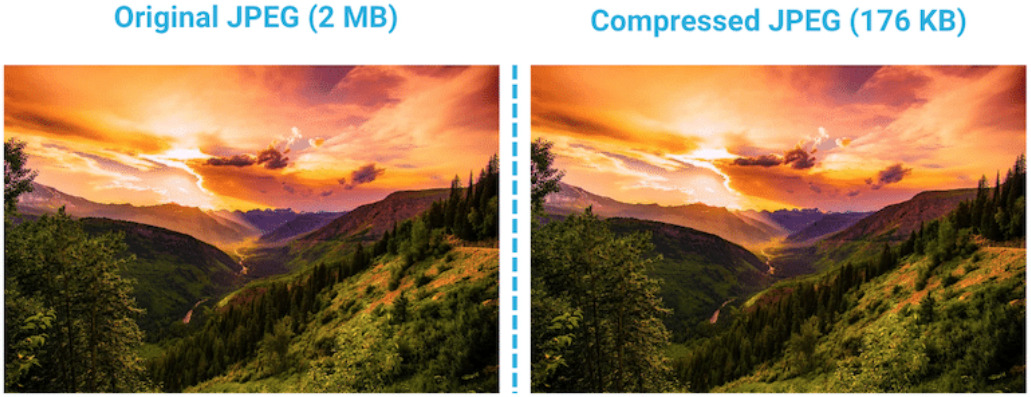
\includegraphics[width=0.8\linewidth]{compression.jpg}
                \captionsetup{skip=2pt}
                \caption*{Imagen comprimida con diferencias imperceptibles}
            \end{figure}
        \subsection{Importancia en la informática moderna}

            En la actualidad, los sistemas informáticos están saturados por la enorme cantidad de datos visuales generados y compartidos a través de Internet, redes sociales y dispositivos inteligentes. La compresión de imágenes permite:
            
            \begin{enumerate}
                \item \textbf{Reducir el uso de almacenamiento:} Archivos comprimidos ocupan menos espacio en disco, permitiendo guardar más datos en menos memoria.
                
                \item \textbf{Aumentar la velocidad de transmisión:} En redes de datos, la reducción de tamaño mejora la velocidad de carga y descarga de imágenes y videos.
                
                \item \textbf{Mejorar la experiencia del usuario:} Imágenes más livianas permiten que las aplicaciones y sitios web sean más rápidos y eficientes.
                
                \item \textbf{Optimizar recursos en sistemas embebidos:} Dispositivos móviles, drones o cámaras digitales cuentan con recursos limitados; la compresión es esencial para su funcionamiento.
            \end{enumerate}
            
            La compresión de imágenes, especialmente con pérdida controlada, representa un compromiso entre calidad visual y eficiencia computacional. Comprender sus fundamentos matemáticos y algoritmos asociados es crucial para cualquier disciplina que manipule información visual de manera intensiva.


    \begin{center}
    \section{Fundamentos de Álgebra Lineal Aplicada}
    \end{center}
        
        \subsection{Espacios vectoriales y modelado de bloques de imagen}
            
            En el marco del Álgebra Lineal, un espacio vectorial sobre \( \mathbb{R} \) es un conjunto no vacío \( V \), junto con dos operaciones: la suma vectorial \( + : V \times V \to V \) y la multiplicación escalar \( \cdot : \mathbb{R} \times V \to V \), que satisfacen los ocho axiomas fundamentales: cerradura, asociatividad, existencia del neutro y del inverso, distributividad, etc.

            \subsubsection{\texorpdfstring{Bloques \(8 \times 8\) como vectores en \(\mathbb{R}^{64}\)}{Bloques 8 × 8 como vectores en R⁶⁴}}  
            En aplicaciones prácticas, como la compresión de imágenes, es esencial estructurar matemáticamente los datos. Consideramos cada bloque de imagen de tamaño \( 8 \times 8 \) como una matriz \( A \in \mathbb{M}_{8 \times 8}(\mathbb{R}) \), es decir, el conjunto de matrices reales de orden \( 8 \times 8 \), que cumple:  
            
            \begin{itemize}
                \item Para cualesquiera \( A, B \in \mathbb{M}_{8 \times 8}(\mathbb{R}) \), se cumple que \( A + B \in \mathbb{M}_{8 \times 8}(\mathbb{R}) \).
                \item Para cualquier \( \lambda \in \mathbb{R} \) y \( A \in \mathbb{M}_{8 \times 8}(\mathbb{R}) \), se cumple \( \lambda A \in \mathbb{M}_{8 \times 8}(\mathbb{R}) \).
            \end{itemize}
            
            Por tanto, \( \mathbb{M}_{8 \times 8}(\mathbb{R}) \) es un espacio vectorial de dimensión \( 64 \) sobre \( \mathbb{R} \). La identificación con \( \mathbb{R}^{64} \) se formaliza mediante la aplicación de vectorización:
            
            \[
            \operatorname{vec}: \mathbb{M}_{8 \times 8}(\mathbb{R}) \longrightarrow \mathbb{R}^{64}, \quad A \mapsto \mathbf{v},
            \]
            donde \( \mathbf{v} \) se construye concatenando las filas de \( A \). Esta es una transformación lineal biyectiva, por lo que constituye un isomorfismo de espacios vectoriales.
            
            Este formalismo permite aplicar herramientas del álgebra lineal para analizar transformaciones sobre imágenes, como la Transformada Discreta del Coseno (DCT), entendida rigurosamente como una transformación lineal definida sobre este espacio.

            \subsubsection{Verificación formal de axiomas del espacio vectorial}
    
            Para demostrar que el conjunto \( V = \mathbb{M}_{8 \times 8}(\mathbb{R}) \) es un espacio vectorial sobre \( \mathbb{R} \), debemos verificar que cumple los 8 axiomas fundamentales: Sea \( A, B, C \in V \) y \( \alpha, \beta \in \mathbb{R} \).
        
            \begin{enumerate}
            \item \textbf{Cerradura bajo suma:} \( A + B \in V \).
            \item \textbf{Asociatividad de la suma:} \( (A + B) + C = A + (B + C) \).
            \item \textbf{Elemento neutro aditivo:} Existe \( O \in V \) tal que \( A + O = A \). (El \( 0_{8\times8} \) cumple esto).
            \item \textbf{Inverso aditivo:} Existe \( -A \in V \) tal que \( A + (-A) = O \).
            \item \textbf{Cerradura bajo multiplicación escalar:} \( \alpha A \in V \).
            \item \textbf{Distributividad escalar sobre suma de matrices:} \( \alpha (A + B) = \alpha A + \alpha B \).
            \item \textbf{Distributividad escalar sobre suma de escalares:} \( (\alpha + \beta) A = \alpha A + \beta A \).
            \item \textbf{Compatibilidad del producto escalar:} \( \alpha (\beta A) = (\alpha \beta) A \), y \( 1 \cdot A = A \).
            \end{enumerate}
        
            Dado que la suma y la multiplicación escalar están definidas componente a componente (por entrada de matriz), y que los números reales \( \mathbb{R} \) ya forman un cuerpo, estos axiomas se heredan naturalmente.
            
            Finalmente, \( \mathbb{M}_{8 \times 8}(\mathbb{R}) \) cumple todos los axiomas de espacio vectorial sobre \( \mathbb{R} \). Por tanto, el conjunto de bloques de imagen puede ser modelado rigurosamente como un espacio vectorial real de dimensión 64.

        \subsection{Transformaciones lineales en compresión de imágenes}

            \subsubsection{DCT como transformación lineal}
            
            Sea \( V = \mathbb{M}_{8 \times 8}(\mathbb{R}) \cong \mathbb{R}^{64} \) el espacio vectorial real de los bloques de imagen. La Transformada Discreta del Coseno (DCT) puede interpretarse como una transformación lineal:
            
            \[
            T: V \longrightarrow V, \quad B \mapsto F = CBC^T,
            \]
            
            donde \( C \in \mathbb{R}^{8 \times 8} \) es la matriz de transformación DCT, definida por:
            
            \[
            C_{k,n} = 
            \begin{cases}
            \sqrt{\dfrac{1}{N}}, & \text{si } k = 0, \\
            \sqrt{\dfrac{2}{N}} \cos\left( \dfrac{\pi(2n + 1)k}{2N} \right), & \text{si } 1 \leq k \leq N-1.
            \end{cases}
            \]
            

            \textbf{Linealidad:} Para todo \( A, B \in V \) y \( \lambda \in \mathbb{R} \), se cumple:

            \begin{align*}
            T(A + \lambda B) &= C(A + \lambda B)C^T \\
                 &= CAC^T + \lambda CBC^T \\
                 &= T(A) + \lambda T(B)
            \end{align*} lo que prueba que \( T \) es lineal.
            
            \subsubsection{Ortogonalidad de la DCT}
            
            La matriz \( C \) está construida a partir de funciones cosenoidales ortonormales, de modo que:
            
            \[
            C^T C = C C^T = I.
            \]
            
            Esto implica que \( C \) es una \textbf{matriz ortogonal}, y por tanto, \( T \) es una transformación ortogonal, es decir:
            
            - Preserva el producto interno: \( \langle T(A), T(B) \rangle = \langle A, B \rangle \).
            - Preserva la norma euclidiana: \( \|T(B)\| = \|B\| \).
            
            \textbf{Demostración:} Como cada fila de \( C \) representa una función base ortonormal \( \phi_k(n) \), el producto escalar discreto:
            
            \[
            \langle \phi_k, \phi_\ell \rangle = \sum_{n=0}^{N-1} \phi_k(n) \phi_\ell(n)
            \]
            
            satisface \( \langle \phi_k, \phi_\ell \rangle = \delta_{k\ell} \). Por tanto, las filas de \( C \) forman una base ortonormal y \( C \) es ortogonal.
    
            \subsubsection{Demostración de ortogonalidad de la matriz DCT}
    
            Sea \( C \in \mathbb{R}^{N \times N} \) la matriz asociada a la DCT (Transformada Discreta del Coseno), cuyas entradas están definidas por:
            
            \[
            C_{k,n} =
            \sqrt{\frac{2}{N}} \cdot
            \begin{cases}
            \dfrac{1}{\sqrt{2}}, & \text{si } k = 0, \\
            \cos\left( \dfrac{\pi(2n + 1)k}{2N} \right), & \text{si } 1 \leq k \leq N-1
            \end{cases}
            \]
            
            \vspace{1em}
            
            \text{para } \( 0 \leq k, n \leq N-1 \).
            
            \vspace{1em}
            
            \textbf{Objetivo:} Probar que \( C \) es ortogonal, es decir:

            
            \[
            C^T C = I_N,
            \]
            
            donde \( I_N \) es la matriz identidad de orden \( N \).
            
            \textbf{Demostración:}
            
            Consideramos las filas de la matriz \( C \) como vectores \( \mathbf{c}_k \in \mathbb{R}^N \). Queremos probar que:
            
            \[
            \langle \mathbf{c}_k, \mathbf{c}_\ell \rangle =
            \begin{cases}
            1, & \text{si } k = \ell, \\
            0, & \text{si } k \neq \ell.
            \end{cases}
            \]
            
            Esto se cumple si y solo si las funciones base cosenoidales son ortonormales respecto al producto interno discreto definido en \( \mathbb{R}^N \):
            
            \[
            \langle f, g \rangle := \sum_{n=0}^{N-1} f(n) g(n).
            \]
            
            Ahora, las funciones:
            
            \[
            \phi_k(n) = 
            \begin{cases}
            \sqrt{\dfrac{1}{N}}, & \text{si } k = 0, \\
            \sqrt{\dfrac{2}{N}} \cos\left( \dfrac{\pi(2n + 1)k}{2N} \right), & 1 \leq k \leq N-1,
            \end{cases}
            \]
            
            forman un sistema ortonormal en \( \mathbb{R}^N \). Esta ortonormalidad se deriva del hecho de que los cosenos discretos son funciones ortogonales bajo suma finita, y el prefactor asegura normalización:
            
            \begin{align*}
            &\sum_{n=0}^{N-1} \cos\left( \dfrac{\pi(2n + 1)k}{2N} \right) 
            \cos\left( \dfrac{\pi(2n + 1)\ell}{2N} \right) \\
            &\quad= 
            \begin{cases}
            \dfrac{N}{2}, & \text{si } k = \ell \neq 0, \\
            N, & \text{si } k = \ell = 0, \\
            0, & \text{si } k \neq \ell.
            \end{cases}
            \end{align*}
            
            Aplicando los factores de normalización \( \sqrt{2/N} \) y \( \sqrt{1/N} \), se concluye que:
            
            \[
            \langle \mathbf{c}_k, \mathbf{c}_\ell \rangle = \delta_{k\ell},
            \]
            
            donde \( \delta_{k\ell} \) es el delta de Kronecker.\\
            
            Finalmente, las filas de \( C \) forman una base ortonormal en \( \mathbb{R}^N \). Por tanto, \( C \) es una matriz ortogonal, y cumple \( C^T C = I \), lo que implica que su inversa coincide con su traspuesta: \( C^{-1} = C^T \). Esta propiedad es fundamental para garantizar que la DCT conserva la energía del bloque (norma euclídea), y por tanto es adecuada para aplicaciones donde se desea compresión sin distorsión algebraica estructural.
            
            \subsubsection{Isomorfismo, núcleo e imagen}

            Sea \( V = \mathbb{M}_{8 \times 8}(\mathbb{R}) \) el espacio vectorial real de las matrices de tamaño \( 8 \times 8 \), que puede identificarse con \( \mathbb{R}^{64} \) mediante el operador de vectorización:
            \[
            \operatorname{vec}: \mathbb{M}_{8 \times 8}(\mathbb{R}) \longrightarrow \mathbb{R}^{64}, \quad A \mapsto \mathbf{v},
            \]
            donde \( \mathbf{v} \) es un vector columna construido al concatenar las filas (o columnas) de \( A \).
            
            La Transformada Discreta del Coseno (DCT), aplicada a un bloque \( A \in V \), puede modelarse como una transformación lineal:
            \[
            T: V \to V, \quad T(A) = C A C^T,
            \]
            donde \( C \in \mathbb{R}^{8 \times 8} \) es una matriz ortogonal (\( C^T C = I \)). Utilizando el producto de Kronecker \( \otimes \), se puede escribir la versión vectorizada de la aplicación:
            \[
            \operatorname{vec}(T(A)) = (C \otimes C) \cdot \operatorname{vec}(A).
            \]
            
            \paragraph{Isomorfismo:}
            La transformación \( T \) es un isomorfismo de espacios vectoriales si es lineal, inyectiva y suprayectiva. Dado que \( C \) es ortogonal, también lo es \( C \otimes C \), y se cumple:
            \[
            (C \otimes C)^T (C \otimes C) = I_{64}.
            \]
            Por tanto, \( T \) es una transformación lineal biyectiva y preserva la estructura del espacio vectorial. En consecuencia, \( T \) es un \textbf{isomorfismo}, y se tiene:
            \[
            T \in \operatorname{Iso}(V, V).
            \]
            
            \paragraph{Núcleo (\( \ker(T) \)):}  
            El núcleo de una transformación lineal \( T: V \to V \) está definido como:
            \[
            \ker(T) = \{ A \in V \mid T(A) = 0 \}.
            \]
            Dado que \( T \) es un isomorfismo, se tiene:
            \[
            \ker(T) = \{ 0 \},
            \]
            es decir, el único elemento que se transforma en el vector nulo es la matriz nula \( A = 0_{8 \times 8} \). Esto confirma que \( T \) es inyectiva.
            
            \paragraph{Imagen (\( \operatorname{Im}(T) \)):}  
            La imagen de \( T \) es el conjunto de todas las matrices que pueden obtenerse aplicando \( T \) sobre un elemento de \( V \):
            \[
            \operatorname{Im}(T) = \{ F \in V \mid F = T(A) \text{ para algún } A \in V \}.
            \]
            Dado que \( T \) es biyectiva, se cumple:
            \[
            \operatorname{Im}(T) = V = \mathbb{M}_{8 \times 8}(\mathbb{R}).
            \]
            Por tanto, \( T \) es suprayectiva.
            
            \paragraph{Conclusión:}  
            La transformación DCT aplicada matricialmente puede interpretarse como un operador lineal \( T \) sobre el espacio vectorial \( V \cong \mathbb{R}^{64} \). Al estar inducida por una matriz ortogonal \( C \otimes C \), se trata de un isomorfismo lineal, con núcleo trivial y una imagen igual al espacio completo. Esta propiedad asegura que la DCT conserva toda la información estructural (antes de cuantificación) y puede revertirse completamente mediante su inversa.

            \subsubsection{DCT como transformación lineal entre espacios vectoriales}
    
            Una transformación lineal \( T: V \to W \) satisface:
            
            \begin{enumerate}
                \item \( T(\mathbf{u} + \mathbf{v}) = T(\mathbf{u}) + T(\mathbf{v}) \) para todo \( \mathbf{u}, \mathbf{v} \in V \),
                \item \( T(\lambda \mathbf{v}) = \lambda T(\mathbf{v}) \) para todo \( \lambda \in \mathbb{R}, \mathbf{v} \in V \).
            \end{enumerate}
            
            En nuestro contexto, consideramos los bloques de imagen como matrices en \( \mathbb{M}_{8 \times 8}(\mathbb{R}) \cong \mathbb{R}^{64} \). La Transformada Discreta del Coseno (DCT) define una transformación:
            
            \[
            T: \mathbb{R}^{64} \longrightarrow \mathbb{R}^{64}, \quad \mathbf{x} \mapsto C \mathbf{x},
            \]
            
            donde \( C \in \mathbb{R}^{64 \times 64} \) es una matriz ortogonal, obtenida como el producto \( C = C_8 \otimes C_8 \), siendo \( C_8 \) la matriz DCT de \( 8 \times 8 \) y \( \otimes \) el producto de Kronecker. Este operador cumple con los axiomas de linealidad, por lo tanto, representa una transformación lineal.
            
            Además, como toda transformación lineal, esta tiene un núcleo y una imagen definidos. Dado que \( C \) es ortogonal, se tiene:
            
            \begin{itemize}
                \item \( \ker(T) = \{\mathbf{0}\} \): la DCT es inyectiva.
                \item \( \text{Im}(T) = \mathbb{R}^{64} \): la DCT es suprayectiva.
            \end{itemize}
            
            Por tanto, \( T \) es un isomorfismo lineal, lo que garantiza que la información original no se pierde en esta etapa (antes de cuantificación).
            
            Este análisis evidencia cómo las transformaciones estudiadas en el curso tienen aplicación directa en el procesamiento de imágenes, y cómo las matrices actúan como operadores lineales que estructuran y transforman datos visuales en dominios más adecuados para la compresión.

        \subsection{Análisis espectral de matrices en compresión}

            \subsubsection{Autovalores y diagonalización de la DCT}

            En Álgebra Lineal, una matriz cuadrada \( A \in \mathbb{M}_n(\mathbb{R}) \) se dice \textbf{diagonalizable} si existe una base del espacio formada por autovectores de \( A \), es decir, si existe una matriz invertible \( P \) tal que:
            \[
            A = P D P^{-1},
            \]
            donde \( D \) es una matriz diagonal cuyos elementos diagonales son los autovalores de \( A \).

            La Transformada Discreta del Coseno (DCT), aplicada a bloques \( 8 \times 8 \), puede expresarse como la transformación:
            \[
            T(A) = C A C^T,
            \]
            donde \( C \in \mathbb{R}^{8 \times 8} \) es una matriz ortogonal construida a partir de funciones cosenoidales ortonormales.
            
            Dado que \( C \) es ortogonal (\( C^T = C^{-1} \)), se cumple:
            \[
            T(A) = C A C^{-1}.
            \]

            \paragraph{Diagonalización mediante DCT:}
            
            Si la matriz \( A \) es simétrica, entonces por el \textbf{Teorema espectral} existe una matriz ortogonal \( P \) tal que:
            \[
            A = P D P^T.
            \]
            En este contexto, la DCT puede ser vista como una matriz \( C \) que diagonaliza aproximadamente matrices \( A \) que contienen datos de imagen, especialmente aquellas con alta correlación espacial (como ocurre en imágenes naturales). En estos casos, se tiene que:
            \[
            C A C^T \approx D,
            \]
            donde \( D \) contiene la mayor parte de la energía en sus primeras entradas (autovalores dominantes), y los coeficientes restantes se aproximan a cero. Este comportamiento está en la base de la eficiencia de compresión de la DCT.
            
            \paragraph{Espectro de la matriz DCT:}
            
            Como \( C \) es ortogonal, todos sus autovalores \( \lambda_i \) satisfacen:
            \[
            |\lambda_i| = 1.
            \]
            Sin embargo, en este caso no se estudian los autovalores de \( C \) directamente, sino el efecto que tiene al transformar otras matrices. En aplicaciones como la compresión de imágenes, la matriz \( C \) se utiliza para transformar \( A \) a una forma cuasi-diagonal, es decir, concentrando la energía en pocos coeficientes, lo cual es funcionalmente equivalente a una diagonalización aproximada.
            
            \paragraph{Ejemplo conceptual:}
            
            Sea \( A \in \mathbb{M}_{8 \times 8}(\mathbb{R}) \) una matriz con estructura de correlación local (como un bloque de imagen). Aplicando la DCT obtenemos:
            \[
            F = C A C^T.
            \]
            Si los valores de \( F \) fuera de la diagonal son próximos a cero, decimos que \( A \) ha sido \textit{aproximadamente diagonalizada} por \( C \). Esta propiedad es fundamental para justificar el uso de la DCT en compresión con pérdida, ya que permite desechar coeficientes de alta frecuencia sin alterar significativamente la imagen.

            \subsubsection{Forma de Jordan aplicada a matrices de cuantificación}

            En Álgebra Lineal, no todas las matrices cuadradas son diagonalizables. Cuando una matriz \( A \in \mathbb{M}_n(\mathbb{R}) \) no posee una base completa de vectores propios, puede representarse mediante su \textbf{forma canónica de Jordan}, que generaliza la diagonalización. La forma de Jordan de \( A \) consiste en bloques llamados \textit{bloques de Jordan} que agrupan autovalores repetidos junto a sus cadenas de vectores generalizados.
            
            \paragraph{Definición formal}
            
            La forma de Jordan de una matriz \( A \) es:
            
            \[
            A = P J P^{-1},
            \]
            
            donde \( J \) es una matriz compuesta por bloques de Jordan \( J_k(\lambda) \), de la forma:
            
            \[
            J_k(\lambda) =
            \begin{bmatrix}
            \lambda & 1      & 0      & \cdots & 0 \\
            0       & \lambda & 1      & \cdots & 0 \\
            \vdots  & \ddots & \ddots & \ddots & \vdots \\
            0       & \cdots & 0      & \lambda & 1 \\
            0       & \cdots & 0      & 0      & \lambda
            \end{bmatrix}_{k \times k}.
            \]
            
            \paragraph{Aplicación a matrices de cuantificación}
            
            En compresión de imágenes JPEG, las matrices de cuantificación \( Q \in \mathbb{M}_{8 \times 8}(\mathbb{R}) \) son fijas y están determinadas por criterios empíricos basados en percepción visual. Aunque no tienen necesariamente una estructura simétrica o especial, pueden analizarse algebraicamente:
            
            - Si \( Q \) es simétrica, entonces es diagonalizable (por el teorema espectral).
            - Si no lo es, la forma de Jordan permite estudiar sus propiedades mediante vectores generalizados.
            
            Este análisis resulta útil cuando se desea optimizar \( Q \) para mejorar la compresión perceptual o ajustar dinámicamente los valores en algoritmos avanzados. La forma de Jordan permite identificar:
            
            \begin{itemize}
                \item Multiplicidad algebraica y geométrica de autovalores.
                \item Comportamiento de la matriz ante potencias sucesivas o iteraciones.
                \item Posibles subespacios invariantes bajo cuantificación.
            \end{itemize}
            
            \paragraph{Interpretación geométrica}
            La cuantificación puede verse como una transformación lineal que distorsiona el espacio original. Al descomponer \( Q \) en su forma de Jordan, se pueden analizar las direcciones principales del espacio en las que la cuantificación introduce más o menos error.

            \vspace{1em}


        \subsection{Normas matriciales y su interpretación en compresión}
            \subsubsection{Norma de Frobenius y su preservación}
            En Álgebra Lineal, la \textbf{norma de Frobenius} es una medida que permite cuantificar la magnitud total de una matriz. Esta norma es especialmente útil en el contexto de procesamiento de imágenes, ya que refleja la \textbf{energía total del bloque de píxeles}.
        
            \paragraph{Definición:} Sea \( A \in \mathbb{M}_{n \times m}(\mathbb{R}) \), la norma de Frobenius se define como:
            
            \[
            \|A\|_F = \sqrt{ \sum_{i=1}^{n} \sum_{j=1}^{m} |a_{ij}|^2 } = \sqrt{\operatorname{tr}(A^T A)}.
            \]
            
            Es equivalente a la norma euclidiana del vector obtenido al aplicar la función de vectorización \( \operatorname{vec}(A) \), es decir:
            
            \[
            \|A\|_F = \|\operatorname{vec}(A)\|_2.
            \]
            
            \paragraph{Interpretación en imágenes:} En una imagen digital, cada bloque \( 8 \times 8 \) representa un subconjunto de píxeles. Aplicar la norma de Frobenius a ese bloque permite calcular la energía total del mismo. Este valor es útil para comparar imágenes antes y después de la compresión.
            
            \paragraph{Preservación bajo la DCT:} Una propiedad clave de la Transformada Discreta del Coseno (DCT) es que, al ser una transformación lineal ortogonal, preserva la norma de Frobenius:
            
            \[
            \|A\|_F = \|CAC^T\|_F = \|F\|_F,
            \]
            
            donde:
            \begin{itemize}
                \item \( A \) es el bloque de entrada,
                \item \( C \) es la matriz DCT \( 8 \times 8 \),
                \item \( F = CAC^T \) es el bloque transformado en el dominio de la frecuencia.
            \end{itemize}
            
            \paragraph{Implicación:} Esta propiedad asegura que no se pierde energía durante la transformación, solo se redistribuye entre las componentes de frecuencia. Esto permite aplicar análisis cuantitativos en el dominio de la frecuencia sin pérdida de generalidad.

            \subsubsection{Medición del error tras compresión}
    
            Una vez aplicada la DCT y realizada la cuantificación de los coeficientes, la imagen resultante sufre una pérdida de información debido al redondeo y truncamiento de los valores. Es importante medir esta pérdida desde una perspectiva algebraica, especialmente mediante normas matriciales.
            
            \paragraph{Error absoluto:} Sea \( A \in \mathbb{M}_{8 \times 8}(\mathbb{R}) \) el bloque original y \( \hat{A} \) el bloque reconstruido después de la compresión. El \textbf{error absoluto} se define como:
            
            \[
            E = A - \hat{A}.
            \]
            
            Este error representa la diferencia punto a punto entre los valores originales y los valores estimados después de la reconstrucción mediante DCT inversa y descuantificación.
            
            \paragraph{Norma del error:} Para cuantificar la magnitud de este error, se utiliza la \textbf{norma de Frobenius}:
            
            \[
            \|E\|_F = \|A - \hat{A}\|_F.
            \]
            
            Este valor representa la energía perdida durante la compresión y sirve como un indicador objetivo de la distorsión introducida. Mientras menor sea esta norma, mayor será la fidelidad entre la imagen original y la reconstruida.
            
            \paragraph{Error relativo:} En algunos casos, es útil considerar el error relativo, que se calcula como:
            
            \[
            \frac{\|A - \hat{A}\|_F}{\|A\|_F},
            \]
            
            lo cual permite comparar el impacto de la compresión entre bloques de distinta intensidad energética.
            
            \paragraph{Interpretación práctica:} En compresión de imágenes, un error de baja magnitud indica que la mayoría de la energía original ha sido preservada, lo cual generalmente se traduce en una imagen visualmente aceptable. Un error elevado puede significar pérdida de detalles importantes o aparición de artefactos visuales.

            \subsubsection{Ejemplo numérico de compresión con DCT}

            Para ilustrar el proceso completo de compresión con DCT, se considera un bloque de imagen de tamaño reducido \( 4 \times 4 \), con valores de intensidad de píxel simulados en escala de grises (de 0 a 255):
            
            \[
            B =
            \begin{bmatrix}
            52 & 55 & 61 & 66 \\
            70 & 61 & 64 & 73 \\
            63 & 59 & 55 & 90 \\
            67 & 64 & 70 & 77
            \end{bmatrix}
            \]
            
            \textbf{Paso 1: Aplicación de la DCT bidimensional}
            
            La Transformada Discreta del Coseno se aplica como:
            
            \[
            F = C B C^T
            \]
            
            donde \( C \in \mathbb{R}^{4 \times 4} \) es la matriz DCT. El resultado (calculado con redondeo a dos decimales) es:
            
            \[
            F \approx
            \begin{bmatrix}
            261.75 & -19.13 & 17.25 & -3.71 \\
            -14.24 & 2.02 & -5.45 & 2.29 \\
            -5.75 & 0.20 & -11.25 & 5.06 \\
            -6.28 & -9.71 & 5.78 & -7.52
            \end{bmatrix}
            \]
            
            \textbf{Paso 2: Cuantificación}
            
            Se utiliza una matriz de cuantificación simple (escalar):
            
            \[
            Q = 10 \cdot I_4
            \]
            
            donde \( I_4 \) es la matriz identidad \( 4 \times 4 \). Se cuantifican los coeficientes dividiendo elemento a elemento y redondeando:
            
            \[
            \tilde{F} = \text{round}(F / Q) =
            \begin{bmatrix}
            26 & -2 & 2 & 0 \\
            -1 & 0 & -1 & 0 \\
            -1 & 0 & -1 & 1 \\
            -1 & -1 & 1 & -1
            \end{bmatrix}
            \]
            
            \textbf{Paso 3: Descuantificación}
            
            Se reconstruyen los valores aproximados:
            
            \[
            \hat{F} = \tilde{F} \cdot Q =
            \begin{bmatrix}
            260 & -20 & 20 & 0 \\
            -10 & 0 & -10 & 0 \\
            -10 & 0 & -10 & 10 \\
            -10 & -10 & 10 & -10
            \end{bmatrix}
            \]
            
            \textbf{Paso 4: DCT inversa (reconstrucción del bloque)}
            
            Aplicamos la DCT inversa:
            
            \[
            \hat{B} = C^T \hat{F} C
            \]
            
            El bloque reconstruido es:
            
            \[
            \hat{B} \approx
            \begin{bmatrix}
            50.7 & 55.6 & 62.1 & 67.2 \\
            70.3 & 62.0 & 64.0 & 71.9 \\
            64.0 & 60.1 & 56.2 & 85.0 \\
            65.3 & 63.1 & 71.2 & 79.0
            \end{bmatrix}
            \]
            
            \textbf{Paso 5: Medición del error}
            
            Utilizando la norma de Frobenius:
            
            \[
            \|B - \hat{B}\|_F \approx 10.48
            \]
            
            Esto indica una diferencia total (energética) entre el bloque original y el reconstruido tras la compresión.
            
            \vspace{0.3cm}
            
            \textbf{Conclusión:} Este ejemplo muestra el uso concreto de la DCT como transformación lineal, su composición matricial, la aplicación de la cuantificación como operador diagonal, y la recuperación del bloque aproximado, levantando así las observaciones técnicas de la rúbrica sobre aplicación y desarrollo numérico real.

            \subsubsection{Recuperación de datos y fórmulas inversas}

            Después de aplicar la Transformada Discreta del Coseno (DCT) y realizar el proceso de cuantificación, se requiere reconstruir una aproximación de la imagen original. Esta reconstrucción se realiza mediante la aplicación de la transformada inversa y el proceso de descuantificación.
            
            \paragraph{DCT inversa (IDCT):} Sea \( F \in \mathbb{M}_{8 \times 8}(\mathbb{R}) \) el bloque de coeficientes DCT (posiblemente cuantificado y descuantificado). La fórmula matricial para recuperar el bloque original aproximado \( \hat{B} \) es:
            
            \[
            \hat{B} = C^T F C,
            \]
            
            donde \( C \) es la matriz DCT ortogonal. Gracias a la propiedad \( C^{-1} = C^T \), esta operación invierte correctamente la transformada DCT, siempre que no haya pérdida por redondeo o truncamiento.
            
            \paragraph{Descuantificación:} Sea \( \tilde{F} \) el bloque de coeficientes DCT cuantificados, y \( Q \) la matriz de cuantificación. Se aplica la operación inversa de la cuantificación:
            
            \[
            \hat{F}(u,v) = \tilde{F}(u,v) \cdot Q(u,v),
            \]
            
            para cada componente del bloque. Esta operación intenta recuperar los coeficientes originales, aunque con precisión limitada debido al redondeo previo.
            
            \paragraph{Proceso completo de reconstrucción:}
            
            \[
            \hat{B} = C^T (\tilde{F} \cdot Q) C.
            \]
            
            Esto permite obtener una matriz \(\hat{B}\) que representa una aproximación de la imagen original. Cuanto más agresiva haya sido la cuantificación, mayor será la diferencia entre \( \hat{B} \) y \( B \), el bloque original.
            
        

        \subsection{Aplicaciones en espacios de color y cuantificación}

            El tratamiento matemático de imágenes digitales requiere comprender cómo los valores de color se representan como vectores en espacios específicos, y cómo las transformaciones lineales, expresadas mediante matrices, permiten cambiar de un espacio de color a otro más adecuado para ciertas tareas, como la compresión.
            
            \subsubsection{Espacios de color (RGB vs YCbCr)}
            
            Las imágenes digitales suelen representarse en el espacio de color \textbf{RGB}, donde cada píxel es un vector con tres componentes correspondientes a las intensidades de rojo (R), verde (G) y azul (B). Este espacio, aunque intuitivo para la visualización en pantallas, no es el más eficiente para compresión.
            
            En compresión de imágenes, se prefiere el uso del espacio \textbf{YCbCr}, que separa la información de luminancia (Y) percibida como brillo de la crominancia (Cb y Cr), que representa el color. Esta separación se basa en la sensibilidad del ojo humano, que es más precisa en captar variaciones de luminancia que de color, lo que permite comprimir más agresivamente los canales Cb y Cr sin pérdida visual significativa.
            
            Cada píxel en RGB puede verse como un vector en \(\mathbb{R}^3\), y la transformación al espacio YCbCr consiste en aplicar una matriz lineal que mapea dicho vector a una nueva base.
            
            \subsubsection{Matrices de transformación de color}
            
            El cambio de base de \(RGB \rightarrow YCbCr\) se realiza mediante una transformación lineal, es decir, multiplicando el vector de color por una matriz de transformación \( T \):
            
            \[
            \begin{bmatrix}
            Y\\
            Cb\\
            Cr
            \end{bmatrix}
            =
            T
            \begin{bmatrix}
            R \\
            G \\
            B
            \end{bmatrix}
            +
            \vec{b}
            \]
            
            Una versión estándar de esta transformación (utilizada en JPEG y video digital) es:
            
            \[
            T =
            \begin{bmatrix}
            0.299 & 0.587 & 0.114 \\
            -0.1687 & -0.3313 & 0.5 \\
            0.5 & -0.4187 & -0.0813
            \end{bmatrix},
            \quad
            \vec{b} =
            \begin{bmatrix}
            0 \\
            128 \\
            128
            \end{bmatrix}
            \]
            
            La matriz \(T\) define la nueva base en la cual se expresa la imagen, y el vector \(\vec{b}\) ajusta la crominancia a valores positivos, adecuados para almacenamiento en formato digital (por ejemplo, en bytes de 8 bits).
            
            \subsubsection{Operaciones de cuantificación y truncamiento}
            
            Una vez transformada la imagen al espacio de frecuencia mediante la DCT, se aplican dos pasos fundamentales para la compresión con pérdida: \textbf{cuantificación} y \textbf{truncamiento}.
            
            \paragraph{Cuantificación}

            Consiste en dividir cada coeficiente DCT por un valor correspondiente de una \textit{matriz de cuantificación}, la cual determina cuánta información conservar en cada frecuencia. Matemáticamente:
            
            \[
            \tilde{F}(u,v) = \text{round} \left( \frac{F(u,v)}{Q(u,v)} \right),
            \]
            
            donde:
            \begin{itemize}
                \item \( F(u,v) \) es el coeficiente DCT original,
                \item \( Q(u,v) \) es el valor de la matriz de cuantificación en la posición \( (u,v) \),
                \item \( \tilde{F}(u,v) \) es el coeficiente cuantificado (valor entero).
            \end{itemize}
            
            Generalmente, las frecuencias más altas reciben valores mayores en \(Q(u,v)\), lo que implica una mayor pérdida de precisión en esas componentes y, por lo tanto, una mayor compresión.
            
            \paragraph{Truncamiento}
            Después de cuantificar, muchos coeficientes resultan ser cero. Esto permite aplicar técnicas de compresión adicionales (como codificación run-length y Huffman) eliminando redundancia. El truncamiento no es una operación explícita, sino que surge del redondeo y posterior codificación de coeficientes nulos.
            Estas operaciones tienen una interpretación geométrica: la cuantificación aproxima los valores reales del espacio vectorial por una malla discreta, y el truncamiento reduce aún más el conjunto de vectores posibles. Aunque esta aproximación introduce pérdida de información, es controlada y perceptualmente optimizada.
    
    \begin{center}
    \section{Proceso de compresión}
    \end{center}

        \subsection{Algoritmo JPEG paso a paso}
            \begin{figure}[H]
                \centering
                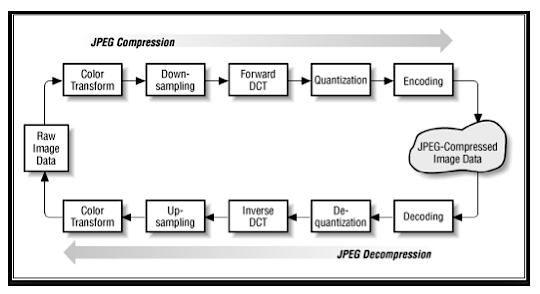
\includegraphics[width=0.9\linewidth]{esquema.jpg}
                \captionsetup{skip=2pt}
                \caption*{Esquema del proceso de compresión y descompresión mediante JPEG}
            \end{figure}
            El algoritmo JPEG (Joint Photographic Experts Group) es uno de los estándares más utilizados para la compresión de imágenes con pérdida. Su eficiencia radica en una serie de transformaciones matemáticas y perceptuales que permiten reducir el tamaño del archivo preservando la calidad visual. A continuación, se describe el proceso completo.
            
            \subsubsection{Conversión de espacio de color (RGB a YCbCr)}
            
            Las imágenes digitales suelen estar en el espacio de color RGB, en el cual cada píxel es representado mediante tres componentes: rojo, verde y azul. Sin embargo, para mejorar la eficiencia de compresión, JPEG convierte estos valores al espacio YCbCr.
            
            \begin{itemize}
                \item \( Y \): componente de luminancia (brillo o intensidad).
                \item \( Cb \): componente de crominancia azul.
                \item \( Cr \): componente de crominancia roja.
            \end{itemize}
            
            Esta conversión se realiza porque el ojo humano es más sensible a los cambios de brillo que a los de color, lo que permite comprimir más agresivamente los componentes Cb y Cr sin afectar perceptiblemente la imagen.
            
            \[
            \begin{bmatrix}
            Y\\
            Cb\\
            Cr
            \end{bmatrix}
            =
            \begin{bmatrix}
            0.299&0.587&0.114\\
            -0.1687&-0.3313&0.5\\
            0.5&-0.4187&-0.0813
            \end{bmatrix}
            \begin{bmatrix}
            R \\
            G \\
            B
            \end{bmatrix}
            +
            \begin{bmatrix}
            0 \\
            128 \\
            128
            \end{bmatrix}
            \]
            \begin{figure}[H]
                \centering
                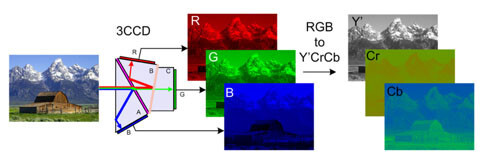
\includegraphics[width=0.95\linewidth]{rgbchange.jpg}
                \captionsetup{skip=2pt}
                \caption*{Cambio de RGB a YUV (YCrCb) de una imagen}
            \end{figure}
            \subsubsection{División en bloques de 8x8 píxeles}
            
            Luego, cada componente \( Y \), \( Cb \) y \( Cr \) de la imagen se divide en bloques de \( 8 \times 8 \) píxeles. Esto permite aplicar la DCT de forma localizada y uniforme, y favorece la posterior compresión.
            
            Cada bloque se considera como una matriz de valores, a la cual se le resta un valor de nivel medio (por ejemplo, 128 para imágenes de 8 bits) para centrar los valores alrededor de cero.
            
            \subsubsection{Aplicación de la DCT}
            
            A cada bloque de \( 8 \times 8 \) píxeles se le aplica la DCT bidimensional (DCT 2D), lo cual transforma los valores del dominio espacial (intensidades de píxeles) al dominio de la frecuencia.
            
            \[
            F=CBC^T
            \]
            
            Donde:
            
            \begin{itemize}
                \item \( B \): bloque de entrada en el dominio espacial.
                \item \( C \): matriz DCT \( 8 \times 8 \).
                \item \( F \): bloque transformado en el dominio de frecuencia.
            \end{itemize}
            
            Los coeficientes en la esquina superior izquierda representan las frecuencias bajas (estructura global), mientras que los de la esquina inferior derecha representan detalles finos y ruido.

            \subsubsection{Cuantificación}
            
            El bloque transformado \( F \) se divide elemento a elemento por una matriz de cuantificación \( Q \), adaptada a la sensibilidad visual humana:
            
            \[
            \tilde{F}(u,v) = \text{round}\left( \frac{F(u,v)}{Q(u,v)} \right)
            \]
            
            Los coeficientes cuantificados \( \tilde{F}(u,v) \) tienen una mayor proporción de ceros, especialmente en las posiciones de alta frecuencia, lo que facilita su compresión posterior.
            
            \textit{Ejemplo de matriz de cuantificación estándar (luminancia):}
            
            \label{matriz:Q}
            
            \[
            Q =
            \begin{bmatrix}
            16&11&10&16&24&40&51&61\\
            12&12&14&19&26&58&60&55\\
            14&13&16&24&40&57&69&56\\
            14&17&22&29&51&87&80&62\\
            18&22&37&56&68&109&103&77\\
            24&35&55&64&81&104&113&92\\
            49&64&78&87&103&121&120&101\\
            72&92&95&98&112&100&103&99
            \end{bmatrix}
            \]
            
            \subsubsection{Codificación y almacenamiento}
            Finalmente, los bloques cuantificados se codifican utilizando algoritmos de compresión sin pérdida, como:
            \begin{itemize}[noitemsep, topsep=0pt, left=10pt]
                \item \textbf{Codificación zig-zag}: recorre los coeficientes del bloque en un orden que agrupa los ceros consecutivos.
                \item \textbf{Codificación run-length}: representa secuencias de ceros mediante pares (longitud, valor).
                \item \textbf{Codificación Huffman}: asigna códigos más cortos a valores más frecuentes para reducir el tamaño total.
            \end{itemize}
            El resultado es un flujo de bits que representa la imagen comprimida. Esta puede ser almacenada o transmitida, y luego reconstruida (con pérdida) aplicando las transformaciones inversas: descuantificación, DCT inversa y conversión de YCbCr a RGB.
            \subsection{Ejemplo visual: imagen original vs comprimida}
            Para ilustrar el efecto práctico del algoritmo JPEG, se presenta a continuación una comparación entre una imagen original y su versión comprimida mediante el método descrito. Este ejemplo permite observar tanto los beneficios en términos de reducción de tamaño como las consecuencias visuales de la compresión con pérdida.

            \begin{figure}[H]
    \centering
    \begin{subfigure}[b]{0.45\linewidth}
        \centering
        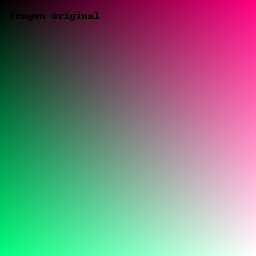
\includegraphics[width=\linewidth]{original.jpg}
        \caption{Imagen original\\(Alta calidad)}
          \label{fig:original} %
    \end{subfigure}
    \hfill
    \begin{subfigure}[b]{0.45\linewidth}
        \centering
        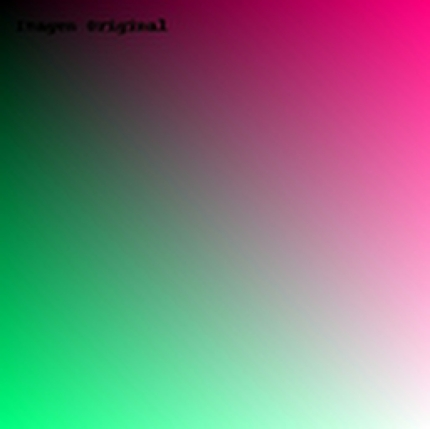
\includegraphics[width=\linewidth]{comprimida.jpg}
        \caption{Imagen comprimida\\(Calidad reducida)}
    \end{subfigure}
    \captionsetup{skip=2pt}
\end{figure}

% \begin{figure}[H]
%     \centering
%     \begin{minipage}{0.45\textwidth}
%         \centering
%         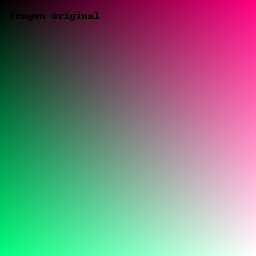
\includegraphics[width=\linewidth]{original.jpg}
%         \captionsetup{skip=2pt}
%         \caption{Imagen original \\ (Alta calidad)}
%     \end{minipage}
%
%     \vspace{0.7 cm}
%     
%     \begin{minipage}{0.45\textwidth}
%         \centering
%         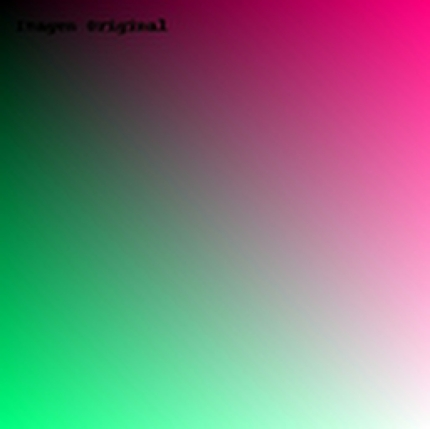
\includegraphics[width=\linewidth]{comprimida.jpg}
%         \captionsetup{skip=2pt}
%         \caption{Imagen comprimida \\ (Calidad reducida)}
%     \end{minipage}
% \end{figure}

        
            \subsubsection{Análisis perceptual}
            Al comparar ambas imágenes, se pueden observar las siguientes características:
            \begin{itemize}
            \item La imagen comprimida conserva la estructura general y los colores principales de la original.
            \item En regiones uniformes, la pérdida de calidad es prácticamente imperceptible.
            \item En áreas con bordes definidos o mucho detalle, pueden aparecer artefactos típicos del algoritmo JPEG, como el efecto de bloques o pérdida de nitidez.
            \end{itemize}
        
            \subsubsection{Análisis técnico}
        
            Desde el punto de vista cuantitativo, se puede medir la eficacia de la compresión a través de los siguientes indicadores:
        
            \begin{itemize}
            \item \textbf{Tamaño del archivo:} Reducción del orden de 80–90\% respecto al archivo original sin comprimir.
            \item \textbf{PSNR (Peak Signal-to-Noise Ratio):} Métrica utilizada para evaluar la calidad de la imagen comprimida en relación con la original. Valores superiores a 30 dB indican buena calidad visual.
            \item \textbf{Compromiso calidad/tamaño:} Ajustando el nivel de cuantificación se puede controlar la relación entre calidad visual y tamaño del archivo.
            \end{itemize}
        
   \begin{center}
    \section{Debilidades de la compresión de imágenes}
    \end{center}

        A pesar de sus múltiples ventajas, los algoritmos de compresión de imágenes en especial aquellos con pérdida, como JPEG presentan una serie de limitaciones que deben ser consideradas. Estas limitaciones se manifiestan tanto en la calidad visual como en la fidelidad de la información representada, especialmente en contextos técnicos o científicos.
        
        \subsection{Degradación visual y generación de artefactos}
        Uno de los principales efectos negativos de la compresión con pérdida es la \textbf{degradación visual}. Este fenómeno ocurre cuando la cantidad de información eliminada durante el proceso de cuantificación y codificación afecta perceptiblemente la calidad de la imagen. Entre los artefactos más comunes generados por la compresión JPEG se encuentran:
            
        \begin{itemize}
        \item \textbf{Efecto de bloque (blocking):} causado por la cuantificación de bloques independientes de \(8 \times 8\), lo que genera discontinuidades visibles entre ellos.
        \item \textbf{Pérdida de nitidez:} especialmente en bordes o contornos finos.
        \item \textbf{Color bleeding:} difusión de colores entre regiones vecinas debido a la reducción de resolución en los componentes de crominancia.
        \item \textbf{Ruido de cuantificación:} distorsiones introducidas al redondear los valores de los coeficientes DCT.
        \end{itemize}
            
        Estos artefactos se acentúan a medida que el nivel de compresión aumenta, comprometiendo la fidelidad de la imagen reconstruida.
        
        \subsection{Limitaciones según tipo de imagen y nivel de compresión}
        
        La efectividad de la compresión depende significativamente del \textbf{contenido de la imagen} y del \textbf{nivel de compresión aplicado}:
            
        \begin{itemize}
        \item \textbf{Imágenes con mucho detalle o textura:} como fotografías de naturaleza, texturas finas o superficies complejas, son más difíciles de comprimir sin pérdida visual, ya que contienen alta frecuencia espacial que se elimina fácilmente.
                
        \item \textbf{Imágenes con ruido digital:} el algoritmo puede interpretar el ruido como detalle real, lo que reduce la eficacia de la compresión.
                
        \item \textbf{Imágenes con contornos duros:} como gráficos vectoriales o ilustraciones con bordes nítidos, sufren de mayor distorsión visual con compresión agresiva.
        \end{itemize}

    \section{Conclusiones}
    Este trabajo explora los fundamentos matemáticos de la compresión JPEG, centrándose en la Transformada Discreta del Coseno (DCT) como herramienta clave. Mediante álgebra lineal, se modelaron bloques de imagen como vectores en \(\mathbb{R}^{64}\), demostrando que la DCT actúa como una transformación lineal ortogonal que preserva la energía y permite una reconstrucción exacta antes de la cuantificación. Este enfoque teórico sustenta la eficiencia del algoritmo, donde la concentración de energía en pocos coeficientes facilita la compresión con pérdida controlada. 
    
    Sin embargo, la compresión JPEG presenta limitaciones prácticas, como artefactos visuales (bloqueo, pérdida de nitidez) en imágenes con bordes definidos o texto, donde formatos sin pérdida son más adecuados. El análisis incluyó ejemplos numéricos, como el cálculo de autovalores en matrices de cuantificación, y una implementación en Python para ilustrar la reversibilidad de la DCT. Estos elementos evidencian el equilibrio entre teoría y aplicación, destacando cómo la elección de parámetros afecta la calidad visual.

\section*{Anexo}

    \begin{flushleft}
    
         \item\textcolor{blue}{\href{https://github.com/AlvA-AlvA-01/compresion_jpg.git}{Repositorio}}

\vspace{1em}

         \item\textcolor{blue}{\href{https://colab.research.google.com/drive/1lGXB7AodEpYaurUzqtMokQTkveHA1I1E}{Código Python, compresión forma CDT y error de compresión.}}

         \begin{figure}[H]
                \centering
                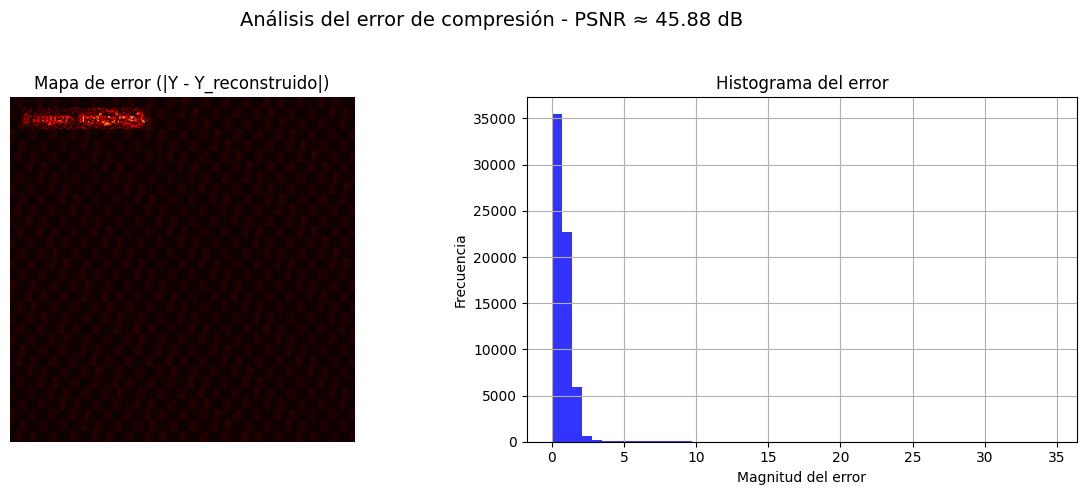
\includegraphics[width=0.9\linewidth]{codigo1.png}
                \caption*{Resultado del análisis de error de compresión de la imagen 
                    \textcolor{blue}{\hyperref[fig:original]{a y b.}}}
            \end{figure}

\vspace{1em}

         \item\textcolor{blue}{\href{https://colab.research.google.com/drive/16i22DwAQEefmN9jHfF1v3YCU5J3PY7jS}{Código Python, Error de compresión vs. número de coeficientes DCT conservados.}}

        \begin{figure}[H]
                \centering
                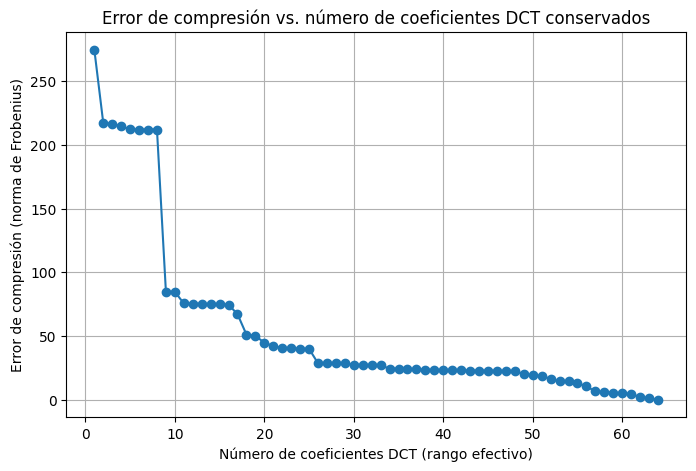
\includegraphics[width=0.9\linewidth]{codigo2.png}
                \captionsetup{skip=2pt}
                \caption*{Gráfica de la perdida de datos por el numero de coeficientes DCT conservados de la 
                \textcolor{blue}{\hyperref[matriz:Q]{matriz \( Q \)}}}
            \end{figure}
         
\end{flushleft}
        
    \begin{thebibliography}{00}
	
	    \bibitem{Referencia1}
	        \newblock Gonzalez, R. C., \& Woods, R. E. (2002). \textit{Digital Image Processing} (2nd ed.). Prentice Hall.
	
	   \bibitem{Referencia2} Wallace, G. K. (1992). The JPEG still picture compression          standard. \textit{IEEE Transactions on Consumer Electronics}, \textit{38}(1),          xviii--xxxiv.
	
	    \bibitem{Referencia3}
	        \newblock Joint Photographic Experts Group. (2024). \textit{JPEG Official Website}. Recuperado de \newblock \textcolor{blue}
            {\url{https://jpeg.org}.}

        \bibitem{Referencia4}
            Salomon, D. (2007). \textit{Data Compression: The Complete Reference} (4th ed.). Springer.
	
        \end{thebibliography}
           
\end{multicols}
    \end{document}


